\documentclass[11pt]{article}
\usepackage[utf8]{inputenc}
\usepackage{fancyhdr}
\usepackage[margin=1.25cm]{geometry}

\title{COMP37111 - Advanced Algorithms I}
\author{Sam Littlefair}

\usepackage{natbib}
\usepackage{graphicx}
\usepackage{hyperref}
\usepackage{enumerate}
\usepackage{amsmath}
\usepackage{textcomp}
\usepackage{lipsum}
\usepackage{algorithm}
\usepackage[noend]{algpseudocode}

\begin{document}

\maketitle

\section{Course Unit Structure}
\begin{itemize}
  \item 10 credit module. Exam worth 75\%.
  \item 2 labs worth 25\%.
  \begin{enumerate}
    \item Coursework A: Due Thursday, 19th October at 12:00 (SSO).
    \item Coursework A: Due Thursday, 23rd November at 12:00 (SSO).
  \end{enumerate}
\end{itemize}

\section{Some Basic Graph Algorithms}
\subsection{Graphs and directed graphs}
\subsubsection{Graphs}
\textbf{Graph:} A graph is a pair G = (V, E), where V is a finite set and E a
set of subsets of V of cardinality 2. \\ \hspace*{14mm} Where V = vertices, E = edges. (Cardinality means number of things in the set.)
\paragraph{Formal notation for a graph:}
\begin{itemize}
    \item If $\{u, v\} \in E$, we say that $u$ and $v$ are neighbours.
    \item If $v \in V$, $e \in E$ and $v \in e$, we say $v$ and $e$ are adjacent.
\end{itemize}
\begin{center}
    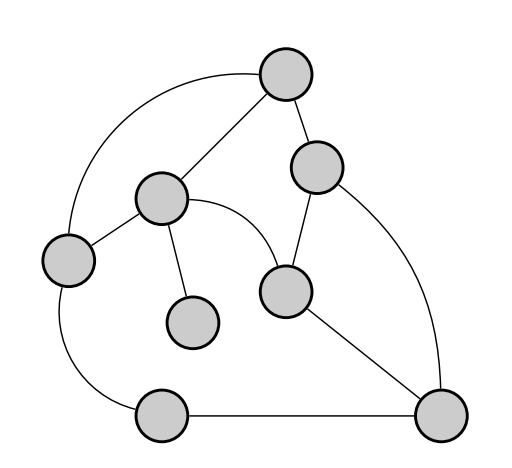
\includegraphics{img/graph.png}
\end{center}
\newpage
\subsubsection{Directed Graphs}
\noindent\textbf{Directed graph:} A pair G = (V, E), where V is a set and E
a set of ordered pairs of distinct elements of V.\\ \hspace*{36mm} Where V = vertices, E = edges, the same as a normal graph.

\begin{center}
    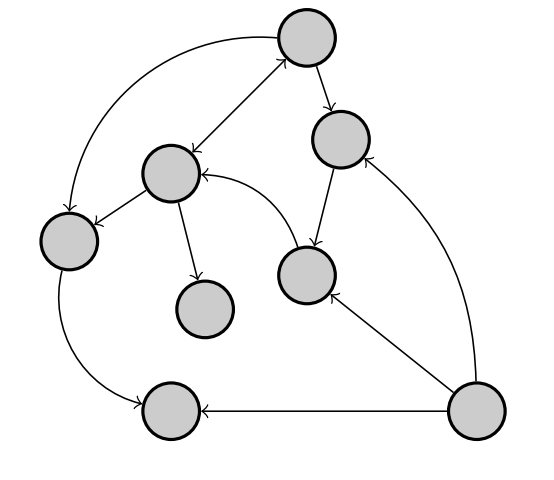
\includegraphics{img/directed_graph.png}
\end{center}

\subsubsection{Graph storage}
\begin{itemize}
    \item A directed graph can be stored using adjacency lists:\\
\end{itemize}
\begin{center}
\newcommand{\sep}{\hspace*{.5em}}
  \noindent
  \begin{tabular}{l}
  Vertex 1 \textrightarrow \hspace{2mm} $\fbox{2} \sep \fbox{3} $\\
  Vertex 2 \textrightarrow \hspace{2mm} $\fbox{1} $\\
  Vertex 3 \textrightarrow \hspace{2mm} $\fbox{1} \sep \fbox{2} \sep \fbox{4} $\\
  Vertex 4 \textrightarrow \hspace{2mm} $\fbox{1} \sep \fbox{3} $\\
\end{tabular}
\end{center}
\begin{itemize}
    \begin{itemize}
        \item From any vertex, the adjacent edges can be accessed efficiently.
        \item From any edge, the adjacent vertices can be accessed efficiently.
    \end{itemize}
\end{itemize}
\bigskip
\begin{itemize}
    \item An undirected graph can be stored using a symmetric matrix:\\
\end{itemize}
\[
\bordermatrix{ & V1 & V2 & V3 & V4 \cr
      V1 & * & 0 & 1 & 1\cr
      V2 & 0 & * & 1 & 1\cr
      V3 & 0 & 0 & * & 1\cr
      V4 & 1 & 1 & 0 & *} \qquad
\]
\begin{itemize}
    \begin{itemize}
        \item Wasteful in memory but more convenient.
    \end{itemize}
\end{itemize}
\newpage
\subsubsection{Graph definitions}
\noindent\textbf{Reachable:} We say that $v$ is reachable from $u$ if there is a path between them.\\

\noindent\textbf{Connected:} A graph is connected if every node is reachable from every other.\\

\noindent\textbf{Strongly Connected:} A directed graph is strongly connected if every vertex is reachable from every other.

\begin{tabbing}
\textbf{Connected Component:} \=A connected component of a graph is a maximal set of vertices \\ \> each of which is reachable from any other.
\end{tabbing}

\begin{tabbing}
\textbf{Strongly Connected Component:} \=A strongly connected component of a directed graph is a maximal set of\\ \>vertices each of which is reachable (in the directed graph sense) from any other.\\
\end{tabbing}

\begin{tabbing}
\noindent\textbf{Cycle:} \=A cycle in a directed graph G is a sequence of vertices $v0, . . . , vk = v0 (k \geq 2)$ such that, for all i\\ \>$(0 \leq i \lessthan k),(vi, vi+1)$ is an edge. Just a fancy way of saying there is a loop between some vertices.\\
\end{tabbing}

\noindent\textbf{Cyclic/Acyclic:} We call a graph cyclic if it has a cycle, otherwise it's acyclic.

\bigskip
\subsubsection{Some problems}
Given the definitions above, how can we compute the following functions?

\begin{algorithm}
\caption{Connected Components}\label{}
\begin{algorithmic}[1]
\State \textbf{Input} A graph G = (V, E).
\State \textbf{Return} The connected components of G.
\end{algorithmic}
\end{algorithm}
\begin{algorithm}
\caption{Strongly Connected Components}\label{}
\begin{algorithmic}[1]
\State \textbf{Input} A graph G = (V, E).
\State \textbf{Return} The strongly connected components of G.
\end{algorithmic}
\end{algorithm}
\begin{algorithm}
\caption{Cyclicity}\label{}
\begin{algorithmic}[1]
\State \textbf{Input} A directed graph G = (V, E).
\State \textbf{Return} True if G is cyclic, False otherwise.
\end{algorithmic}
\end{algorithm}

\newpage
%\section{Depth First Search (DFS)}
\end{document}
